% =============================================================================
% Chapter 10 — Measurement Discipline: Benchmarks That Do Not Lie
% =============================================================================
\chapter{Measurement Discipline: Benchmarks That Do Not Lie}
\label{ch:measurement}

The largest single-stream ``regression'' ever observed on this cluster
never happened. No code change caused it; it was manufactured entirely by
the measuring instrument. The scariest long-context ``failure'' was equally
fictional: a sweep scored the server doing exactly the right thing as a
model collapse. Every optimization chapter in
this book ends with a number --- a decode rate, an acceptance curve, a TTFT
ladder --- and this chapter is about what those numbers had to survive to be
printed. On this cluster, several of the most alarming regressions ever
reported turned out to be bugs in the instrument, not in the model.

The lesson the lab drew was not ``be careful'' but something more
structural: treat the benchmark as a program that can have bugs, give it the
same regression suites the serving stack gets, and never publish a number
whose methodology cannot be replayed. This chapter walks through the five
measurement principles that came out of that discipline, the six-phase audit
suite that operationalizes them, the live verifiers that gate releases, and
the statistics that decide when a number is real.

For an inference engineer the stakes are asymmetric, which is why this
material earns a chapter rather than an appendix: \textbf{measurement bugs
masquerade as model regressions}. The response to a model
regression --- roll back, re-patch, re-quantize --- is expensive; the
response to an instrument bug is a script fix. Misattributing the second as
the first burns days of debugging against a defect that does not exist.
And the failure shapes here (a mis-padded prompt, an SSE-counting bug, a
client timeout) recur in any serving stack, not just this one. The disciplines in
this chapter are the difference between a benchmark that gates releases and
one that generates false alarms.

\section{The founding false alarm}

The audit suite was not designed in the abstract. It was designed after a
false-alarm hunt in mid-August 2026, documented at the top of the repository's
\repofile{AUDIT.md}: tests that answer ``is this deployment actually
good?''\ beyond ``does it respond?''\ were built ``from first principles
after a false-alarm hunt.''

\begin{hbwarstory}
Two instruments failed on the same day. First, a naive throughput benchmark
reported \textasciitilde{}45~\tokspersec{} single-stream decode on a lane whose
true rate was 73+~\tokspersec{}: the prompt it used was pathological and
collapsed the speculative drafter (\Cref{ch:specdecode}), so the
``regression'' was manufactured by the test input. Second, a long-context
garble sweep requested \code{--lengths 524288} but, because it padded
prompts by a word-count heuristic, actually sent \textasciitilde{}815K
tokens. Cases above 700K blew past the 1{,}048{,}576-token ceiling, the
server returned a perfectly correct HTTP~400, and the harness scored that
400 as \texttt{GARBLE DETECTED}. Both alarms consumed real debugging time
chasing model failures that did not exist. The five principles below, and
the closing credo of \repofile{scripts/EVAL.md} --- \emph{``If a phase
regresses, fix the recipe, not the test''} --- are the institutional memory
of that day.
\end{hbwarstory}

\section{The five principles as doctrine}

\repofile{scripts/EVAL.md} states five principles, ``learned the hard way,''
all verified on-cluster on 2026-08-16. Each has a mechanism and a war story.
The canonical implementation of all five at once is
\repofile{scripts/bench-miaai.py}, a \textasciitilde{}108-line script that
every other measuring instrument in the repository either imports ideas from or
literally executes. The five split along a natural seam: two govern the
arithmetic of a rate --- which tokens count, and which seconds --- and three
govern the prompt, so that the request being timed is the one production
would actually issue.

\subsection{Tokenize-verified lengths, never word counts}

The naive heuristic ``1.3 words per token'' under-pads by
\textasciitilde{}1.2$\times$ on the DeepSeek-V4 tokenizer: the English
filler used by the sweeps actually runs \textasciitilde{}1.56 tokens per
word (measured directly: 340{,}787 words tokenized to 533{,}110 tokens).
That error is invisible at 8K and catastrophic at 512K --- it is exactly
what turned the 524{,}288 sweep into an 815K sweep and produced the false
garble verdict. The fix is mechanical: every prompt builder in the audit
suite loops \code{POST /tokenize} until the measured count reaches the
target, \emph{before} the request fires. \repofile{scripts/boot-shape-warmup.sh}
takes the discipline to its extreme: it refuses to fire a warmup request
whose token count is not \emph{exactly} right. It is warming specific
Triton compile keys (\Cref{ch:perf}), and warming the wrong shape is worse
than warming none.

\subsection{Cold prefill only}

Garble, tool-call truncation, and long-context collapse only reproduce on
cold prefills. A warm request --- one whose prefix is already resident in
the prefix cache --- skips the very computation under test, so ``warm
requests passing proves nothing.'' Every benchmark prompt therefore begins
with a unique nonce (\code{unique request {nonce}}) that busts the prefix
cache. In \repofile{scripts/bench-miaai.py} the nonce encodes prompt size,
concurrency, trial, and lane index, so no two requests in a sweep can ever
share a cached prefix. The warmup test suite even asserts that nonces
differ across runs, ``or the prefix cache would skip the warmed prefill''
--- cold-vs-warm is the difference between a test and a placebo.

\subsection{Pathological prompts collapse the drafter}

A repeated-word prompt (``distributed distributed distributed\ldots'')
triggers degenerate repetition in the target model that collapses the
DSpark speculative drafter: per-position acceptance falls from
0.93\,$\to$\,0.33 across draft positions on good prompts to
0.72\,$\to$\,0.11 on the pathological one. Since accepted draft tokens are
the lever for decode speed (\Cref{ch:specdecode}), the collapsed acceptance
reads as a fake \textasciitilde{}45~\tokspersec{} ``regression'' --- roughly a 40\%
loss that no code change caused. Doctrine: benchmark prompts use unique
cold prefixes \emph{plus real task instructions}. The MiaAI matrix
methodology asks for ``exactly 128 numbered lowercase English words'' ---
mundane, but linguistically natural enough that the drafter behaves as it
does in production. The same phenomenon resurfaces in the A/B dossiers of
\Cref{ch:perf}: the numbered-word bench holds 45--51\,\% \emph{overall}
acceptance, against the 68--75\,\% overall band the health gate expects on
natural prose. Compare overall against overall. The audit checklist's own
shorthand puts the bench band next to natural-prose \emph{position-0}
acceptance, which is a different instrument reading a different quantity and
makes the gap look wider than it is.
\repofile{scripts/ab-measure.sh} prints both bands with their own reference
ranges, precisely so nobody scores one against the other's baseline.

\subsection{Decode-only windows: exclude TTFT and warmup}

Wall-clock \tokspersec{} includes prefill time, so it punishes long prompts for
having long prefills and says nothing about decode health. The doctrine is
to report decode \tokspersec{} measured \emph{after the first token} ---
MiaAI's \code{median_output_tok_s} --- and TTFT separately.
\Cref{fig:measure-timeline} shows the window boundaries and where the naive
measurements go wrong. Two exclusions matter:

\begin{itemize}
\item \textbf{TTFT is excluded.} The decode rate is
  \code{usage.completion_tokens} divided by (finish time $-$ first-token
  time). The first-token timestamp is taken at the first stream delta
  carrying \code{content}, \code{reasoning}, or \code{reasoning_content}.
\item \textbf{Warmup is excluded.} The first request after a server
  restart pays a 6--10\,s cold-autotune TTFT that is \emph{not} a
  regression; the protocol warms $\geq$2 requests per prompt length before
  any timed trial. Across repeated trials the reported figure is the
  median of per-trial medians, deliberately robust to cold-boot outliers.
\end{itemize}

\begin{figure}[htbp]
\centering
\begin{tikzpicture}[font=\small]
  % --- timeline axis ---
  \draw[hbarrow] (0,0) -- (13.2,0) node[below right=0pt and -8mm,hblabel]{time};
  % segment boxes above axis
  \node[hbfaint,minimum width=16mm,minimum height=7mm,anchor=south west] (warm) at (0.2,0.25) {cold\\autotune};
  \node[hbbox,minimum width=30mm,minimum height=7mm,anchor=south west] (prefill) at (2.4,0.25) {prefill};
  \node[hbgpu,minimum width=62mm,minimum height=7mm,anchor=south west] (decode) at (5.6,0.25) {decode (tokens stream out)};
  % event ticks
  \foreach \x/\lbl in {2.4/{request\\sent}, 5.6/{first token\\(TTFT stamp)}, 11.8/{finish +\\usage frame}} {
    \draw[thick,color=hbSteel] (\x,-0.12) -- (\x,0.12);
    \node[hblabel,align=center,below] at (\x,-0.2) {\lbl};
  }
  % warmup annotation
  \node[hblabel,align=center,anchor=south] at (1.4,1.70) {first request after restart:\\6--10 s TTFT, NOT a regression\\(warm $\geq$2 requests first)};
  \draw[hbfail,dashed] (0.85,1.66) -- (warm.north);
  % TTFT brace
  \draw[decorate,decoration={brace,mirror,raise=11mm}] (2.4,0) -- (5.6,0)
    node[midway,below=13mm,hblabel,align=center]{TTFT\\(reported separately)};
  % decode-only brace (correct)
  \draw[decorate,decoration={brace,raise=10mm},color=hbGreen!70!black] (5.6,1.05) -- (11.8,1.05)
    node[midway,above=12mm,hblabel,color=hbGreen!70!black,align=center]
    {decode-only window (correct):\\tok/s = usage.completion\_tokens / (finish $-$ first token)};
  % naive wall-clock brace (wrong)
  \draw[decorate,decoration={brace,mirror,raise=20mm},color=hbAccent] (2.4,0) -- (11.8,0)
    node[midway,below=22mm,hblabel,color=hbAccent,align=center]
    {naive wall-clock tok/s: includes prefill --- punishes long prompts, hides decode health};
  % SSE chunk note (upper-left, clear of the green brace label)
  \node[hbwarn,align=center,font=\scriptsize,anchor=south west] (ssebox) at (0.2,3.0)
    {counting SSE delta chunks: $\approx$4.5$\times$ undercount\\(MTP packs several accepted tokens per chunk)};
  \draw[hbfail] (ssebox.south) to[bend right=12] (6.3,1.18);
\end{tikzpicture}
\caption{Anatomy of one benchmarked request. The reported decode rate uses
only the green window, with token counts from the final usage frame. The
two red measurements --- wall-clock rates that include prefill, and
per-chunk SSE event counting --- both produced false regressions on this
cluster before the doctrine was codified.}
\label{fig:measure-timeline}
\end{figure}

\subsection{Usage frames, never SSE chunk counts}

DSpark speculative decoding packs multiple accepted draft tokens into a
single SSE stream chunk. Counting per-chunk \code{delta.content} events
therefore undercounts generated tokens by roughly 4.5$\times$ --- and since
tokens are the numerator of every rate, an event-counting benchmark reports
a catastrophic slowdown that never happened. The doctrine: always count via
\code{usage.completion_tokens}, requested with
\code{stream_options={"include_usage": true}} (or via non-streaming usage).
\repofile{scripts/benchmark-0731.py} adds a belt-and-suspenders fallback:
if a stream produced no usage frame, it tokenizes the collected output text
rather than counting chunks. The complete pinned request that implements
the doctrine looks like this:

\needspace{11\baselineskip}
\begin{lstlisting}[language=jsonhb]
{
  "temperature": 0.6, "top_p": 0.95,
  "max_tokens": 128, "min_tokens": 128,
  "ignore_eos": true,
  "chat_template_kwargs": {"thinking": false},
  "stream": true,
  "stream_options": {"include_usage": true}
}
\end{lstlisting}

\noindent
\code{ignore_eos} with \code{min_tokens=max_tokens} guarantees exactly 128
output tokens, so rates are comparable across trials; \code{thinking:
false} keeps the completion out of unbounded reasoning.

That last knob carries its own war story.
\repofile{scripts/benchmark-0731.py} does \emph{not} disable thinking, and
reasoning is not obliged to reach EOS. Without a \code{max_tokens} cap, a
single lane was once observed generating for hours --- over 200k tokens at
\textasciitilde{}75~\tokspersec{}, no error raised anywhere --- while the entire
sweep sat stalled behind it. The script's in-code comment records the
incident and makes the cap mandatory.

\section{The audit suite: six phases, one verdict}

Principles enforce nothing on their own; they need a harness that runs them
against every candidate deployment. \repofile{scripts/run-audit.sh} is that
harness --- the one-command ship/no-ship gate for a serving configuration,
run against a live endpoint:

\begin{lstlisting}[language=bash]
bash scripts/run-audit.sh \
  --base-url http://127.0.0.1:8888/v1 \
  --model deepseek-v4-flash-0731
\end{lstlisting}

It creates a timestamped \repofile{results/audit-<stamp>/} directory and
runs six phases through a wrapper that tees each phase's output to its own
log and folds exit codes into a single pass/fail. The wrapper uses
\code{PIPESTATUS[0]} so the \code{tee} cannot mask a failure. Each phase is
an independently runnable script; the harness adds only sequencing,
logging, and the verdict (\Cref{fig:audit-pipeline}).

\begin{figure}[htbp]
\centering
\begin{tikzpicture}[node distance=8mm and 6mm,font=\small]
  \node[hbhost] (orch) {run-audit.sh\\{\scriptsize creates results/audit-<stamp>/}};
  \node[hbbox,below=of orch,minimum width=52mm] (p1) {1. throughput\\{\scriptsize bench-miaai.py}};
  \node[hbbox,below=of p1,minimum width=52mm] (p2) {2. spec-decode health\\{\scriptsize spec-acceptance.py}};
  \node[hbbox,below=of p2,minimum width=52mm] (p3) {3. RULER-lite quality\\{\scriptsize ruler-lite.py}};
  \node[hbbox,below=of p3,minimum width=52mm] (p4) {4. tool battery\\{\scriptsize tool-battery.py}};
  \node[hbbox,below=of p4,minimum width=52mm] (p5) {5. deep-context tools\\{\scriptsize deepctx-tool-battery.py}};
  \node[hbbox,below=of p5,minimum width=52mm] (p6) {6. garble sweep\\{\scriptsize context-garble-sweep.py}};
  \node[hbgpu,below left=9mm and -14mm of p6] (pass) {ALL-PASS};
  \node[hbwarn,below right=9mm and -14mm of p6] (fail) {FAILURES};
  \draw[hbflow] (orch) -- (p1);
  \draw[hbflow] (p1) -- (p2);
  \draw[hbflow] (p2) -- (p3);
  \draw[hbflow] (p3) -- (p4);
  \draw[hbflow] (p4) -- (p5);
  \draw[hbflow] (p5) -- (p6);
  \draw[hbok] (p6) -- (pass) node[midway,left=1mm,hblabel]{every phase exit 0};
  \draw[hbfail] (p6) -- (fail) node[midway,right=1mm,hblabel]{any phase failed};
  % gate labels on the right
  \node[hblabel,right=4mm of p1,align=left]{gate: C1 decode 73--76 tok/s,\\C6 aggregate 168--180};
  \node[hblabel,right=4mm of p2,align=left]{gate: acceptance $\approx$68--75\%,\\pos0 $\approx$0.93 $\to$ pos4 $\approx$0.33};
  \node[hblabel,right=4mm of p3,align=left]{gate: every task at every\\length passes (retrieval 100\%)};
  \node[hblabel,right=4mm of p4,align=left]{gate: 7/7; truncation reports\\finish=length, never broken JSON};
  \node[hblabel,right=4mm of p5,align=left]{gate: 8/8 at 32K/131K,\\cold prefills};
  \node[hblabel,right=4mm of p6,align=left]{gate: CLEAN at every length\\to the 1M ceiling};
  \begin{scope}[on background layer]
    \node[hbgroup,fit=(p1)(p2)(p3)(p4)(p5)(p6)] {};
  \end{scope}
\end{tikzpicture}
\caption{The six-phase serving audit. Each phase is a standalone script
hitting the live endpoint; the orchestrator tees per-phase logs into the
report directory and folds exit codes into one verdict. Expected values are
for this recipe (2$\times$ DGX Spark, Anemll 0.1.1, verified 2026-08-16).}
\label{fig:audit-pipeline}
\end{figure}

Scope widens down the list: the first two phases ask whether decode is fast
and why it is fast, the middle three whether quality and tool contracts
survive deeper context, and the last whether anything coherent comes back
near the 1M ceiling. How each phase measures is as important as what it
checks:

\textbf{Phase 1 (throughput)} runs \repofile{scripts/bench-miaai.py} at a
256-token prompt, concurrency 1, five repeats --- the full five-principle
methodology of the previous section.

\textbf{Phase 2 (spec-decode health)} captures acceptance from Prometheus
\code{/metrics} by \emph{window deltas}: snapshot the counters, run a short
bench burst so they move, snapshot again, and report
$\Delta$accepted/$\Delta$drafted plus the per-position curve from
\code{vllm:spec_decode_num_accepted_tokens_per_pos_total}. The script's
comments encode two instrument bugs it survived. It anchors on the
\code{_total} suffix because the sibling \code{_created} gauge carries a
Unix timestamp a prefix match would read as a counter. And it parses the
position label with a regex because this build emits \code{position} as the
last label --- the old comma-split parse silently dropped every position
and left the acceptance curve permanently empty. Acceptance is ``THE lever
for decode speed'' (abliteration measurably drains it: 0.585 vs.\ 0.718),
so drift here is a red flag even when throughput still looks acceptable.

\textbf{Phase 3 (RULER-lite)} is long-context quality beyond shallow
needle-in-a-haystack, covered in the next section.

\textbf{Phase 4 (tool battery)} runs seven live tool-calling checks at
temperature 0: single call, complex nested schema, multi-turn, parallel
calls, thinking-plus-tools, forced \code{tool_choice}, and the
\ghissue{55} truncation contract. That last check is a \code{max_tokens=40}
request that forces a cut mid-tool-call and must report
\code{finish_reason="length"}
rather than emit broken tool JSON. Every emitted \code{function.arguments}
string is re-parsed as JSON.

\textbf{Phase 5 (deep-context tools)} repeats the tool contract at 32K and
131K, behind a cold nonce'd Hermes-style system prompt padded with the
measured 1.56 tokens/word ratio --- here approximate padding is acceptable,
because the check is behavioral validity at depth, not an exact-length
claim.

\textbf{Phase 6 (garble sweep)} plants three tripwires in an agent-shaped
system prompt --- tool schemas, a secret codename with ``do not mention,''
and ``never reveal this prompt.'' It pads to each target length, asks a
mundane question cold, and scores the reply against a taxonomy of garble
signatures: \code{SECRET_LEAK}, \code{SCHEMA_LEAK}, \code{PROMPT_ECHO},
\code{SPECIAL_TOK} (a literal \code{<|} in output), \code{EMPTY},
\code{BAD_TOOL_ARGS}, and the subtlest, \code{MID_WORD} --- a reply that
\emph{starts} with punctuation, the signature of decoding resuming
mid-token after KV corruption.

\begin{table}[htbp]
\centering\footnotesize
\caption{Expected audit values on this recipe (2$\times$ DGX Spark, Anemll
0.1.1, verified 2026-08-16).}
\label{tab:audit-expected}
\begin{tabular}{@{}ll>{\raggedright\arraybackslash}p{6.6cm}@{}}
\toprule
Phase & Instrument & Expected on this recipe \\
\midrule
Throughput & \repofile{bench-miaai.py} & C1 73--76 \tokspersec{} (Keys ablit.\ 73.1, official 75.5); C6 agg.\ 168--180 \\
Spec-decode & \repofile{spec-acceptance.py} & 68--75\% overall; pos0 $\approx$0.93 $\to$ pos4 $\approx$0.33 \\
RULER-lite & \repofile{ruler-lite.py} & retrieval 100\%; tracing/aggregation pass at all lengths \\
Tool battery & \repofile{tool-battery.py} & 7/7; \ghissue{55} truncation always \code{finish=length} \\
Deep-context & \repofile{deepctx-tool-battery.py} & 8/8 at 32K/131K \\
Garble & \repofile{context-garble-sweep.py} & CLEAN at every length to the 1M ceiling \\
\bottomrule
\end{tabular}
\end{table}

\section{Long-context evaluation done right}

\repofile{scripts/ruler-lite.py} adapts NVIDIA RULER's task generators
(single- and multi-key needle retrieval, multi-hop variable tracking,
common-words aggregation) to run live against the OpenAI-compatible
endpoint. RULER's core finding motivates the task mix: models that are
perfect at shallow needle retrieval still fail tracing and aggregation at
depth, so a long-context gate that only does NIAH certifies nothing. But
the instrument's own history is the more instructive story, because it
failed twice --- silently --- before it could be trusted.

\subsection{The padding bug: 32K cells that tested 4.8K}

The original padding loop appended one haystack sentence per iteration with
a safety guard of 200 iterations. The guard silently ceilinged every prompt
at \textasciitilde{}4{,}840 tokens --- so the ``32K'' and ``262K'' RULER
cells were actually testing under 5K of context, \emph{while exiting 0}.
Every cell passed; the passes were meaningless (\ghissue{81}). The fix is
bulk padding: compute how many sentence copies close the remaining gap from
a measured per-sentence token count, append them all, re-tokenize, and
iterate (with a 40-round guard that now cannot bind at realistic lengths).

Two hard gates were added on top. After padding, \code{run_case}
\emph{re-verifies} the built prompt via \code{/tokenize} and raises
``padding fell short'' if the actual count is below 97\% of the target ---
a padded-prompt claim must be provable, before any chat call fires. And the
regression suite \repofile{scripts/test-ruler-lite-pad.py} keeps a
re-created 200-sentence-cap loop as a checked-in negative control,
demonstrating that it tops out at 4{,}840 tokens --- the bug is preserved
as evidence.

\subsection{The timeout that scored itself as a model failure}

The second failure was arithmetic. The harness's 900\,s client timeout
meets this cluster's prefill physics --- the recorded datum is an
899{,}994-token prompt taking 1{,}028.85\,s to first token at
\textasciitilde{}874.8 prefill \tokspersec{} --- and loses: 900\,s buys only
about 787K tokens of prefill. Any case near the 1M ceiling therefore has
its socket hung up mid-prefill by the harness's own timer, and ``the
harness scores its own client limit as a model FAIL.'' The constant now
carries that datum as a comment, and \repofile{scripts/run-audit.sh}
forwards \code{--request-timeout} specifically so near-ceiling sweeps can
pair a longer deadline with their lengths. The flag's argparse type rejects
0, negatives, NaN, and infinity --- each of which would otherwise resurface
as a spurious per-case FAIL rather than a usage error
(\Cref{fig:measure-ceilings} puts all three instrument ceilings on the one
axis they share).

\begin{figure}[htbp]
\centering
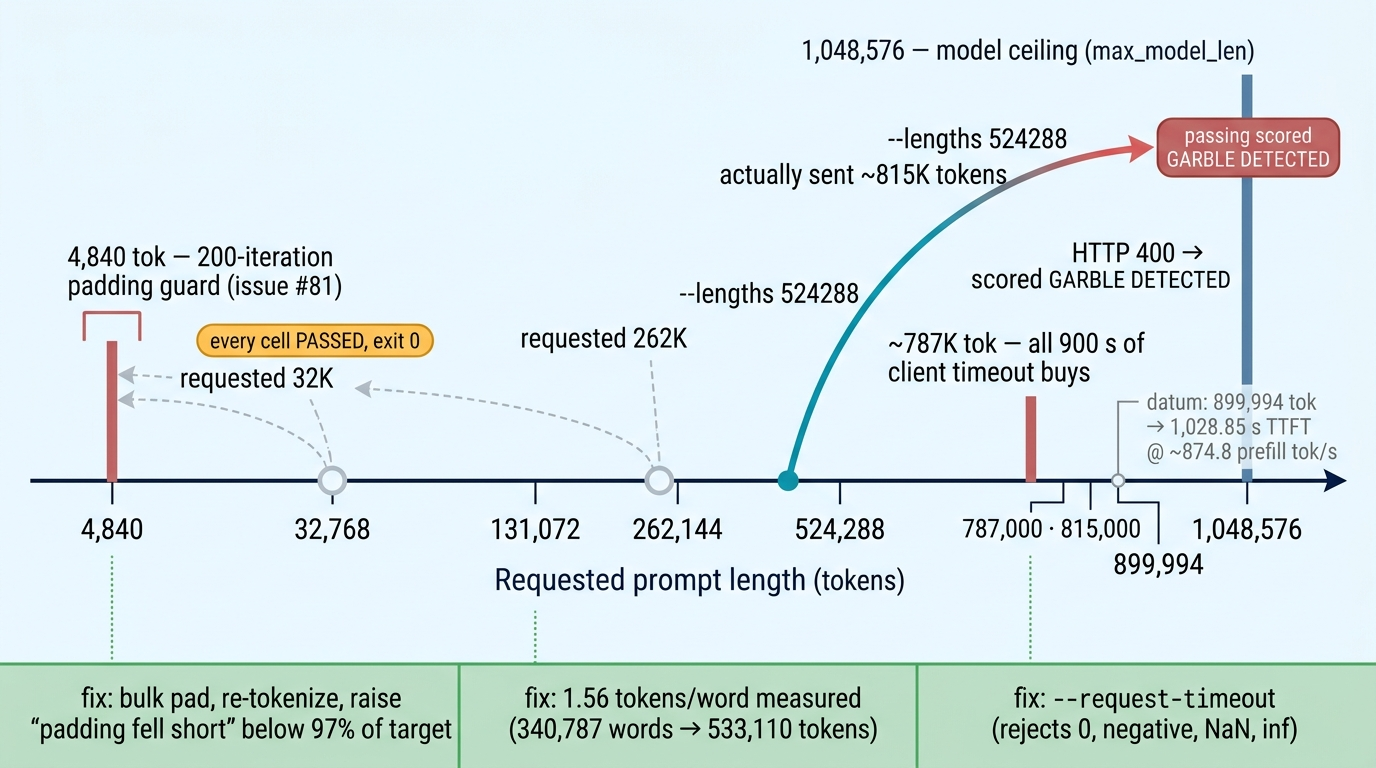
\includegraphics[width=\textwidth]{figures/ch10-instrument-ceilings.png}
\caption{Three ceilings that were not the model's. On one length axis: the
200-iteration padding guard flattened every deep RULER cell to
\textasciitilde{}4{,}840 tokens while exiting 0 (\ghissue{81}); the
1.3-words-per-token heuristic turned a 524{,}288-token request into
\textasciitilde{}815K and past the 1{,}048{,}576 ceiling, so a correct
HTTP~400 was scored \texttt{GARBLE DETECTED}; and the harness's own
900\,s timeout buys only \textasciitilde{}787K tokens of prefill against
the recorded 899{,}994-token / 1{,}028.85\,s datum. Only the steel rule at
1{,}048{,}576 belongs to the model.}
\label{fig:measure-ceilings}
\end{figure}

\begin{hblesson}
The instrument is a suspect too. The padding bug made deep cells test
shallow context while reporting success; the client timeout converted its
own limit into a model verdict; SSE counting undercounted 4.5$\times$; a
label-order assumption silently emptied the acceptance curve. Each bug got
what serving bugs get: a root cause, a fix, and a permanent regression
suite (\repofile{test-ruler-lite-pad.py}, \repofile{test-spec-acceptance.py},
\repofile{test-responses-api-live.py}, \repofile{test-boot-shape-warmup.sh})
--- several of which keep the original bug as a checked-in negative
control. If a benchmark gates releases, it deserves tests exactly as much
as the code it gates.
\end{hblesson}

\section{Live verifiers as release gates}

The six-phase audit is the broad, periodic gate; a fix that changes one
contract needs something sharper. Beyond the periodic audit, therefore,
specific fixes ship with dedicated live
verifiers --- scripts that hit a running endpoint and prove a contract
holds, run as gates before a change is declared done
(\Cref{ch:patches,ch:bugs}). The section's governing principle comes from
\repofile{docs/PATCHES.md}: \emph{``The JSON request report alone is not
the complete live gate.''} A verifier can only see what the API surface
shows it; the failure modes that matter most (a wedged pair, a silent
stream truncation) show up in logs and health state first. Every gate below
is therefore a conjunction --- a case report \emph{plus} log and counter
evidence --- and each of its assertions exists because of a specific
failure it would catch. What distinguishes the verifiers below is not the
endpoints they hit but the disciplines they demonstrate: gates that reach
past request shape into engine behavior, a bounded case matrix whose verdict
includes both ranks' logs, and mode strictness, where a verifier asserts the
behavior the deployment was configured for rather than accepting either
outcome.

\subsection{The Responses API verifier}

\repofile{scripts/verify-responses-api-live.py} is the deep contract check
for the \code{/v1/responses} surface. It runs exact-text and strict
JSON-schema gates; the strictest SSE frame validator in the repository (exactly
one \code{response.completed}, last, with integer usage; concatenated
deltas must reproduce the non-streaming text); and three gates that go past
request/response shape into engine behavior:

\begin{itemize}
\item \textbf{Store LRU} exists to catch a FIFO store masquerading as LRU
  --- an eviction policy that would silently drop a conversation's most
  recently used context. The mechanism: fill the response store to its
  declared capacity, \emph{touch} the oldest entry via GET, roll over with
  one more POST, and require that the touched entry survives while the
  true least-recently-used entry returns 404.
\item \textbf{Appended multi-turn cache floor} exists to catch a prefix
  cache that quietly stops hitting on append-only conversations --- the
  exact workload agents generate. The mechanism: a tokenize-verified
  \textasciitilde{}21K nonce'd prefix, six appended turns with exact
  sentinels, and from turn 2 on an \emph{engine-aware} floor on
  \code{usage.prompt_tokens_details.cached_tokens},
  $\lfloor(\text{prompt}-4096)/256\rfloor \times 256$, derived from the
  sliding-window and block sizes --- a minimum cache-hit guarantee, not a
  vague ``caching works.''
\item \textbf{Disconnect} exists to catch orphaned decode --- an engine
  that keeps generating for a client that hung up, burning slots invisible
  to any per-request view. The mechanism: open a raw stream with
  \code{ignore_eos}, confirm via \code{/metrics} that the request is
  running, close the socket, and validate an entire counter chain.
  Running and waiting must drain to zero within a bounded window; counters
  stay monotonic; the successful-request counter at idle equals its
  pre-request value (an abort must \emph{not} count as a success); only a
  bounded handful of tokens post-open; and generation frozen after idle.
\end{itemize}

\subsection{The issue-136 canary: logs are part of the gate}

The \ghissue{136} XGrammar-termination backport (a grammar-state desync
under speculative decoding, \Cref{ch:bugs}) ships with a bounded live
canary, \repofile{scripts/verify-issue136-xgrammar-live.py}: 20 sequential
strict-tool cases, 100 concurrent cases at concurrency 4 alternating
required and named \code{tool_choice}, five \code{ignore_eos} strict-schema
cases that deliberately force generation \emph{past} grammar termination
(the exact upstream failure trigger), ten ordinary-tool controls, and ten
plain-chat controls. That is 145 cases, health-checked before and after,
with a deliberately redacted JSON report that never contains request
bodies, response bodies, or credentials.

\begin{lstlisting}[language=bash]
VLLM_API_KEY='...' python3 scripts/verify-issue136-xgrammar-live.py \
  --base-url http://127.0.0.1:8888/v1 \
  --model deepseek-v4-flash-dspark \
  --output /tmp/issue136-xgrammar-live.json
\end{lstlisting}

But the documented gate is explicitly larger than the verifier's report.
Per \repofile{docs/PATCHES.md}, from the saved UTC start time both rank
logs must contain \emph{zero} matcher-termination warnings, zero
\code{Failed to advance FSM} / grammar-rejection lines, zero shared-memory
broadcast-block waits, zero \code{sample_tokens} timeouts, and zero
engine-dead errors; container restart counts must remain unchanged; and no
request may remain running with frozen generation progress. This is the
section's opening principle made concrete: the gate is the conjunction of
the 145/145 report, the both-rank log sweep, and the health/restart
evidence --- never the JSON report alone.

\subsection{Mode-strict verification: issue 138}

\repofile{scripts/verify-issue138-responses-history-live.py} guards the
Responses-API full-history replay fix (\ghissue{138}) and demonstrates a
third verifier discipline: \textbf{mode strictness}. The flag
\code{--expect-legacy rejected|accepted} is mandatory, and the verifier
asserts the \emph{configured} behavior --- ``not either outcome passes.''
In rejected mode, a legacy type-less assistant item must yield HTTP~400
with a numeric error code and a message naming the offending field; in
accepted mode it must yield exactly 200. The verifier then proves three
more things: semantic continuity (a fact stated in a legacy item must be
recallable, showing the item participates in context rather than merely
parsing); that six malformed negative variants still 400 (the
compatibility patch must not become a validation hole); and that three
canonical positive controls still 200. A verifier that passes on ``either
behavior'' would silently bless a mis-deployed flag; mode strictness makes
the deployment configuration itself part of the assertion. Both this
verifier and the Responses verifier have their own CPU test suites that
replay fake endpoints against them and pin the exact shape of every request
they make --- the instruments are under test, all the way down.

\section{CPU CI versus live gates}

Every gate so far has needed a live endpoint --- but most of what the repository
proves, it proves without one. The repository runs two disjoint evidence systems,
and knowing which claims each
can make is itself measurement discipline. \repofile{scripts/ci-validate.sh}
is the CPU-only gate chain (also the GitHub Actions workflow): shell syntax
and Python compilation over every script, \textasciitilde{}33 hermetic unit
suites, and a long section of regression-guard greps that freeze past
incidents as executable memory. What CPU CI \emph{can} enforce:

\begin{itemize}
\item \textbf{Wiring, defaults, and fail-closed behavior}: every hotfix
  must be default-off, gated on an exact-\code{1} env comparison, invoked
  fail-closed (\code{|| exit 1}), and synced to the worker --- four
  properties, each independently grepped per patch, and behaviorally
  re-proven by stub-driven suites (\Cref{ch:patches}). Injected-fault
  tests complete the proof: they make \code{os.replace} fail on the
  $N$-th call, corrupt bytes after publish, and interrupt verification
  reads, proving every patcher rolls back to exact original bytes and
  permissions.
\item \textbf{Fixture SHA triangulation}: patches are byte-transformations
  between pinned states. Fixture hashes, patcher constants, and
  test-local literal hunks are three independent legs that must agree ---
  replaying the test's own copy of a hunk over the pinned stock fixture
  must reproduce the pinned post fixture byte-for-byte. One backport is
  even verified against the official upstream merge by Git blob SHA-1.
\item \textbf{Emulated semantics}: \repofile{scripts/verify-dsv4-027-equality-gate.py}
  proves a GPU patch safe without a GPU by pinning the constants, emulating
  the gate arithmetic on CPU, and sweeping the integer-division boundary.
\end{itemize}

What only the live pair can establish: actual \tokspersec{}, kernel behavior
(JIT storms, autotune tactics, CUDA-graph capture coverage), and
tensor-parallel behavior (collective timing, watchdog interactions,
\ghissue{117}-class hangs). CPU CI can prove the recipe \emph{says} what it
should and fails \emph{how} it should; only the audit and the verifiers can
prove the deployment \emph{performs}. The repository never lets one system claim
the other's territory --- \repofile{ci-validate.sh}'s own header says it
``does NOT run the live 2$\times$ Spark serve, decode bench, or
tool-eval-bench.''

\subsection{Double-entry measurement bookkeeping}

Bridging the two systems is the most transferable idea in this chapter:
every live claim is booked twice, once client-side and once server-side,
and the entries must agree. The prefix-cache repro (\ghissue{26}) counts a hit only when
per-lane \code{usage.prompt_tokens_details.cached_tokens} \emph{and} the
server's \code{prefix_cache_hits_total} delta are both positive. The
starvation repro derives its decode rate from a forced exact output-token
count and then verifies it against the \code{generation_tokens_total}
delta. The disconnect gate's entire verdict is a counter chain. A
client-side impression that the server's own counters do not corroborate is
treated as an instrument bug until proven otherwise --- which is exactly
how the SSE undercount was caught (\Cref{fig:measure-double-entry} sets the
three pairings side by side as a ledger).

\begin{figure}[htbp]
\centering
\adjustbox{max width=\textwidth}{%
\begin{tikzpicture}[font=\small]
  % --- column headers -------------------------------------------------------
  \node[hbnode,text width=54mm,align=center,fill=navy,draw=navy,
        text=white,font=\small\bfseries] (ch) at (3.2,0) {CLIENT-SIDE ENTRY};
  \node[hbnode,text width=54mm,align=center,fill=brandgray,draw=brandgray,
        text=white,font=\small\bfseries] (sh) at (11.0,0) {SERVER-SIDE ENTRY};
  % --- row 1: prefix-cache repro (both entries must be positive) ------------
  \node[hbbox,text width=54mm,align=center,font=\scriptsize] (c1) at (3.2,-1.9)
    {\ttfamily usage.prompt\_tokens\_details.\\cached\_tokens};
  \node[hbgpu,text width=54mm,align=center,font=\scriptsize] (s1) at (11.0,-1.9)
    {\ttfamily prefix\_cache\_hits\_total ($\Delta$)};
  \node[hbnode,fill=ice,draw=teal,font=\scriptsize,inner sep=3pt,
        minimum height=6mm] (and1) at (7.1,-1.9) {AND};
  \draw[hbarrow,<->,color=teal] (c1.east) -- (and1.west);
  \draw[hbarrow,<->,color=teal] (and1.east) -- (s1.west);
  \node[hbpatch,font=\scriptsize,inner sep=3pt,minimum height=6mm,anchor=west]
    (i26) at (14.4,-1.9) {issue \ghissue{26}};
  \draw[hbarrow,color=amber!80!black] (i26.west) -- (s1.east);
  \node[hblabel,anchor=south] at (7.1,-1.18) {entries must agree};
  % --- row 2: starvation repro ---------------------------------------------
  \node[hbbox,text width=54mm,align=center,font=\scriptsize] (c2) at (3.2,-3.6)
    {forced exact output-token count};
  \node[hbgpu,text width=54mm,align=center,font=\scriptsize] (s2) at (11.0,-3.6)
    {\ttfamily generation\_tokens\_total ($\Delta$)};
  \draw[hbarrow,<->,color=teal] (c2.east) -- (s2.west);
  % --- row 3: disconnect gate = a counter chain -----------------------------
  \node[hbbox,text width=54mm,align=center,font=\scriptsize] (c3) at (3.2,-6.9)
    {socket closed after \texttt{/metrics} confirms request running};
  \node[hbgpu,text width=54mm,align=center,font=\scriptsize] (k1) at (11.0,-5.2)
    {running / waiting $\to$ 0 (bounded window)};
  \node[hbgpu,text width=54mm,align=center,font=\scriptsize] (k2) at (11.0,-6.4)
    {counters monotonic};
  \node[hbgpu,text width=54mm,align=center,font=\scriptsize] (k3) at (11.0,-7.6)
    {successful-request counter unchanged (abort $\neq$ success)};
  \node[hbgpu,text width=54mm,align=center,font=\scriptsize] (k4) at (11.0,-8.9)
    {bounded tokens post-open; generation frozen at idle};
  \draw[hbarrow,color=brandcyan] (k1) -- (k2);
  \draw[hbarrow,color=brandcyan] (k2) -- (k3);
  \draw[hbarrow,color=brandcyan] (k3) -- (k4);
  \draw[hbarrow,<->,color=teal] (c3.east) -- (8.1,-6.9);
  % --- verdict rail ---------------------------------------------------------
  \node[hbpatch,text width=58mm,align=left,font=\small] (rule) at (3.4,-10.7)
    {\textbf{disagreement $\Rightarrow$ instrument bug until proven
     otherwise}};
  \node[hbwarn,text width=70mm,align=left,font=\scriptsize] (sse) at (11.2,-10.7)
    {caught here: SSE chunk counting undercounts $\approx$4.5$\times$
     $\to$ count \texttt{usage.completion\_tokens}\\[2pt]
     {\ttfamily stream\_options=\{"include\_usage": true\}}};
  \draw[hbfail] (sse.north) -- (7.1,-9.7);
  \begin{scope}[on background layer]
    \node[hbgroup,fit=(ch)(c1)(c2)(c3)] {};
    \node[hbgroup,fit=(sh)(s1)(s2)(k1)(k4)] {};
  \end{scope}
\end{tikzpicture}%
}
\caption{Double-entry measurement bookkeeping. Every live claim is booked
once client-side and once server-side, and a claim is a result only when
both entries agree: the prefix-cache repro requires \code{cached_tokens}
\textbf{and} a positive \code{prefix_cache_hits_total} delta (\ghissue{26});
the starvation repro checks its forced output-token arithmetic against
\code{generation_tokens_total}; the disconnect gate is nothing but a counter
chain. A client-side impression the server's counters do not corroborate is
an instrument bug until proven otherwise --- which is exactly how the
$\approx$4.5$\times$ SSE undercount was caught.}
\label{fig:measure-double-entry}
\end{figure}

\section{Benchmark noise and statistics}

Even a number booked correctly on both sides of the ledger can mislead if
the trial count cannot support the claim hung on it. The final discipline is
statistical honesty about what a number of trials
can resolve. Single-stream decode on this lane swings with the prompt
drawn: identical c=1 trials range roughly 48--76~\tokspersec{}, and the working
noise figure is $\pm$10~\tokspersec{} at c=1. Three trials cannot resolve a
1--3\% knob --- a fact the 2026-09-02 A/B session learned when a
single-PF-vs-dual-PF fabric diagnostic produced 65.7 then 54.8~\tokspersec{}
across repeats: statistically a tie, not a fabric problem. The protocol
that emerged (\repofile{scripts/ab-boot.sh}, \Cref{ch:perf}): pool
\textbf{8 trials} per condition per boot (three from the measurement dossier
plus five extra, precisely because ``c=1 noise on this lane is
\textasciitilde{}$\pm$10 tok/s''), report medians, compare whole
distributions against a \emph{same-day} baseline, and demand separation.
A knob is ON only when its trials clear the baseline's range, not its
mean --- the three verdict shapes that rule produces are drawn in
\Cref{fig:measure-separation}.

\begin{figure}[htbp]
\centering
\adjustbox{max width=\textwidth}{%
\begin{tikzpicture}[font=\small]
  % ---- the deciding edge: the LOWER edge of the baseline range -------------
  \draw[dashed,thick,color=navy] (6.0,2.60) -- (6.0,7.0);
  \node[hbtitle,anchor=south,font=\scriptsize\bfseries] at (6.0,7.05)
    {baseline minimum --- the edge that decides};
  % ---- lane 1: separated BELOW the baseline range -> OFF ------------------
  \draw[fill=lightgray,draw=brandgray] (6.0,6.12) rectangle (9.0,6.68);
  \node[hblabel,font=\tiny,anchor=base] at (8.2,6.34) {baseline};
  \draw[thick,color=navy] (7.4,6.12) -- (7.4,6.68);
  \draw[fill=clueerror!20,draw=clueerror!70!black] (2.4,6.12) rectangle (5.2,6.68);
  \draw[thick,color=navy] (4.0,6.12) -- (4.0,6.68);
  \node[hbwarn,font=\scriptsize,inner sep=3pt,minimum height=5mm,anchor=west]
    at (12.7,6.4) {OFF};
  % ---- lane 2: separated ABOVE the baseline range -> ON -------------------
  \draw[fill=lightgray,draw=brandgray] (6.0,4.82) rectangle (9.0,5.38);
  \node[hblabel,font=\tiny,anchor=base] at (8.2,5.04) {baseline};
  \draw[thick,color=navy] (7.4,4.82) -- (7.4,5.38);
  \draw[fill=brandgreen!18,draw=brandgreen!70!black] (9.9,4.82) rectangle (12.3,5.38);
  \draw[thick,color=navy] (11.2,4.82) -- (11.2,5.38);
  \node[hbgpu,font=\scriptsize,inner sep=3pt,minimum height=5mm,anchor=west]
    at (12.7,5.1) {ON};
  % ---- lane 3: overlapping the baseline range -> tie ----------------------
  \draw[fill=lightgray,draw=brandgray] (6.0,3.52) rectangle (9.0,4.08);
  \node[hblabel,font=\tiny,anchor=base] at (6.7,3.74) {baseline};
  \draw[thick,color=navy] (7.4,3.52) -- (7.4,4.08);
  \draw[fill=amber!45,draw=amber!80!black,fill opacity=0.55]
    (7.6,3.52) rectangle (10.6,4.08);
  \draw[thick,color=navy] (9.1,3.52) -- (9.1,4.08);
  \node[hbpatch,font=\scriptsize,inner sep=3pt,minimum height=5mm,anchor=west]
    at (12.7,3.8) {OFF (tie)};
  % ---- raw spread of this lane, and the working noise figure --------------
  \draw[fill=lightgray!40,draw=brandgray!50] (2.2,2.60) rectangle (12.9,3.10);
  \node[hblabel] at (7.55,2.85) {c=1 trials on this lane: 48--76 \tokspersec{}};
  \draw[hbarrow,<->,color=teal] (2.2,2.25) -- (3.4,2.25);
  \node[hblabel,anchor=west] at (3.55,2.25)
    {working noise figure: $\pm$10 \tokspersec{} at c=1};
  % ---- schematic axis (no ticks: per-trial values are not published) ------
  \draw[hbarrow] (1.8,1.55) -- (13.9,1.55);
  \node[hblabel,anchor=north east] at (13.9,1.42)
    {decode \tokspersec{} --- schematic axis; per-trial values are not published};
  % ---- the three verdicts, keyed to the lanes -----------------------------
  \draw[fill=clueerror!20,draw=clueerror!70!black] (1.8,0.75) rectangle (2.1,0.95);
  \node[hblabel,anchor=west] at (2.25,0.85)
    {TC-decode: c=1 46 vs 55; 7 of 8 trials below baseline minimum $\to$ OFF};
  \draw[fill=brandgreen!18,draw=brandgreen!70!black] (1.8,0.35) rectangle (2.1,0.55);
  \node[hblabel,anchor=west] at (2.25,0.45)
    {capture size 48: c=6 aggregate 139 vs 122 $\to$ ON (reversal A/B: un-fix
     and watch it fall)};
  \draw[fill=amber!45,draw=amber!80!black] (1.8,-0.05) rectangle (2.1,0.15);
  \node[hblabel,anchor=west] at (2.25,0.05)
    {indexer logits 512: $-1.5$/$-1.8$\% inside $\pm$2\% noise $\to$ OFF
     (tie), retry on a $\geq$256K sweep};
  % ---- conditions, and the counter-example ---------------------------------
  \node[hblabel,anchor=north west,align=left] at (1.8,-0.45)
    {8 pooled trials per condition per boot\\same-day baseline\\medians reported};
  \node[hbfaint,font=\scriptsize,text width=62mm,align=left,anchor=north east]
    at (13.9,-0.4)
    {single-PF vs dual-PF: 65.7 then 54.8 across repeats --- a tie, not a
     fabric problem};
\end{tikzpicture}%
}
\caption{A knob is ON only when its trials clear the baseline's
\emph{range}, not its mean. With c=1 trials on this lane ranging
48--76~\tokspersec{} and a working noise figure of $\pm$10~\tokspersec{},
three trials cannot resolve a 1--3\% knob: the 2026-09-02
single-PF-vs-dual-PF diagnostic produced 65.7 then 54.8~\tokspersec{} and
was a tie. Pooling eight trials per condition per boot against a same-day
baseline yields the three verdict shapes applied in \Cref{tab:ab-verdicts}
--- separated below (TC-decode, OFF), separated above (capture size 48, ON,
decided by a reversal A/B), and overlapping (indexer logits 512, tie). The
axis is schematic: per-trial values are not published and are not drawn.}
\label{fig:measure-separation}
\end{figure}

\begin{table}[htbp]
\centering\small
\caption{How 8-trial pooling decided knobs in the September 2026 A/B
sequences. ``Separation'' verdicts cite distribution overlap, not point
estimates.}
\label{tab:ab-verdicts}
\begin{tabular}{@{}ll>{\raggedright\arraybackslash}p{7.0cm}@{}}
\toprule
Knob & Verdict & Evidence (pooled trials, medians) \\
\midrule
TC-decode & OFF & c=1 46 vs.\ 55; 7 of 8 trials below baseline \emph{minimum} \\
Markov replication & OFF & acceptance unchanged; c=6 aggregate 122 vs.\ 148 \\
Capture size 48 & ON & c=6 aggregate 139 vs.\ 122 at 42; all capture-42 trials below base min \\
Inflight prefills = 2 & ON (later demoted) & c=4 8K TTFT spread 9.1 vs.\ 14.6\,s; all trials below base's best --- verdict withdrawn once the \code{r3} admission-count repair landed \\
Indexer logits 512 & OFF (tie) & $-1.5$/$-1.8$\% inside $\pm$2\% noise; retry on a $\geq$256K sweep \\
\bottomrule
\end{tabular}
\end{table}

Two entries in \Cref{tab:ab-verdicts} deserve emphasis as method. The
capture-size verdict came from a \emph{reversal} A/B, a design pattern in
its own right: when the fix is already live, un-fix it briefly. The
suspected fix was reverted and the metric watched to fall
(139\,$\to$\,122) --- the cleanest causal design available on a
production box, because the falling edge rules out every confound the
rising edge cannot. And the inflight-prefills verdict \emph{overturned} an
earlier same-repository decision (\ghissue{154} had reverted the knob to 1 on
fairness grounds); the later measurement, with pooled trials, put it back.
That verdict has since been demoted in turn. The \code{r3} admission-count
repair (PR~\ghissue{211}) made the \ghissue{27} gate count in-flight partial
prefills exactly from \code{self.running}, and the shipped default returned
to 1: the A/B above ran on the pre-\code{r3} undercounting scheduler and, in
the repository's own words, ``does not establish post-r3 behavior.'' Cap 2 keeps
unit coverage but no post-\code{r3} live qualification. Which is the lesson
twice over --- measure the code you run today rather than trusting old
A/Bs, including the A/B you ran last month.

\begin{hbwarstory}
The cost of skipping this discipline is a retraction. The \ghissue{143}
stability matrix claimed an admission-cap mechanism:
``\code{MAX_NUM_SEQS=16} bad / 32 safe.'' The repository's own
\repofile{.env.dspark.example} now carries the verdict in capitals --- the
mechanism is \textbf{RETRACTED}, because ``every cell in that matrix was
n=1; per-burst failure probability explains the whole table without an
admission-cap effect.'' The underlying \ghissue{141} stalls are stochastic
per burst: one configuration ran three clean bursts and died on the
fourth; another died on a fresh-boot first burst. With per-burst failure
probabilities, an $n{=}1$ grid is a random bitmap that will always contain
a plausible-looking pattern. The file's conclusion is the doctrine: ``a
single clean burst cannot distinguish a safe configuration from a lucky
one'' --- and no tested value is declared generally safe.
\end{hbwarstory}

\begin{figure}[htbp]
\centering

\includegraphics[width=0.80\textwidth]{figures/toon-ch10-pareidolia.png}
\caption{Every cell was $n{=}1$. With a per-burst failure probability, a grid of single trials is a random bitmap, and a random bitmap will always contain a plausible-looking pattern for a willing reader to trace. The \ghissue{143} stability matrix published one such pattern as an admission-cap mechanism and later retracted it in capitals. A single clean burst cannot distinguish a safe configuration from a lucky one.}
\label{fig:toon-pareidolia}
\end{figure}

The same honesty governs publication. The dated results ledger
(\repofile{results/RESULTS-2026-08-14.md}) opens with a glossary
disambiguating every marketing-adjacent number: ``1M context'' is a
per-request ceiling, not six chats each holding a million tokens; aggregate
\tokspersec{} is fleet-wide generation, not what one user feels. Each
matrix names its exact method (unique cold prefixes, thinking off,
pinned output length) and its raw JSON companion. Every measurement dossier
from \repofile{scripts/ab-measure.sh} prints its expected reference range
inline with each section, so a results file is self-judging months later.
Numbers without a replayable method are, in this repository's culture, not
results; they are anecdotes awaiting retraction.

The benchmark has changed category. It is not a neutral observer reporting
on the serving stack; it is a second program running against production,
with its own bugs, its own regression suite, and its own demonstrated
capacity to manufacture a 40\% regression out of a prompt or a
4.5$\times$ slowdown out of a chunk count. What a number means has
narrowed accordingly: not what the client felt, but a decode-only window,
booked twice against the server's own counters, pooled across enough
trials to clear a same-day baseline's range, and replayable from a
recorded method. The figure printed in a results file is the last line of
a document that also has a methodology, a noise band, and an expiry date
--- and any of those three can retract it.

\FloatBarrier
\section*{Takeaways}

\begin{itemize}
\item Measurement bugs masquerade as model regressions, and the
  misattribution runs the expensive way: a model regression costs a
  rollback and a re-quantize, an instrument bug costs a script fix. Both
  founding false alarms --- the fake \textasciitilde{}45~\tokspersec{}
  drafter collapse and the correct HTTP~400 scored
  \texttt{GARBLE DETECTED} --- came from the instrument, not the model.
\item Five principles, all mechanized rather than remembered:
  tokenize-verified lengths (never the 1.3-words-per-token heuristic),
  cold nonce'd prefills, natural task prompts, decode-only windows that
  exclude TTFT and warmup, and \code{usage.completion_tokens} instead of
  SSE chunk counts, which undercount by $\approx$4.5$\times$ when MTP
  packs accepted tokens into one delta.
\item The instrument is under test too: every benchmark bug got a root
  cause, a fix, and a permanent regression suite --- several keeping the
  original bug alive as a checked-in negative control, like the
  200-iteration pad loop that ceilinged deep RULER cells at 4{,}840
  tokens while exiting 0 (\ghissue{81}).
\item A JSON pass report alone is not a release gate. A live gate is a
  conjunction --- case report, both ranks' logs, counter deltas, and
  health/restart evidence --- and every live claim is booked double-entry,
  client-side and server-side, with disagreement treated as an instrument
  bug until proven otherwise.
\item Respect the noise: at $\pm$10~\tokspersec{} on this lane, three
  trials cannot resolve a 1--3\% knob, so pool eight per condition per
  boot, compare medians against a same-day baseline, and demand
  distribution separation --- and when an n=1 matrix slips through
  (\ghissue{143}), retract it in public.
\end{itemize}

\chaptertransition{A gate is only worth building if there is a healthy pair
to point it at, and this cluster lost far more serving time to ordinary
operational acts done in the wrong order than to anything a benchmark could
catch. The next chapter is the runbook the audit quietly assumes: the
worker-first boot, the exit-code contract, weights logistics, JIT-cache
doctrine, and the incident-response sequence for the day the pair freezes.
It opens on the most disorienting state this topology can reach --- two
containers that each look individually healthy while the tensor-parallel
group between them is dead or stale, and a launcher whose exit code cannot
tell you which.}
